\newgeometry{top=1cm, bottom=2cm}
\section{Lineare Gleichungssysteme}
\begin{figure}[h!]
    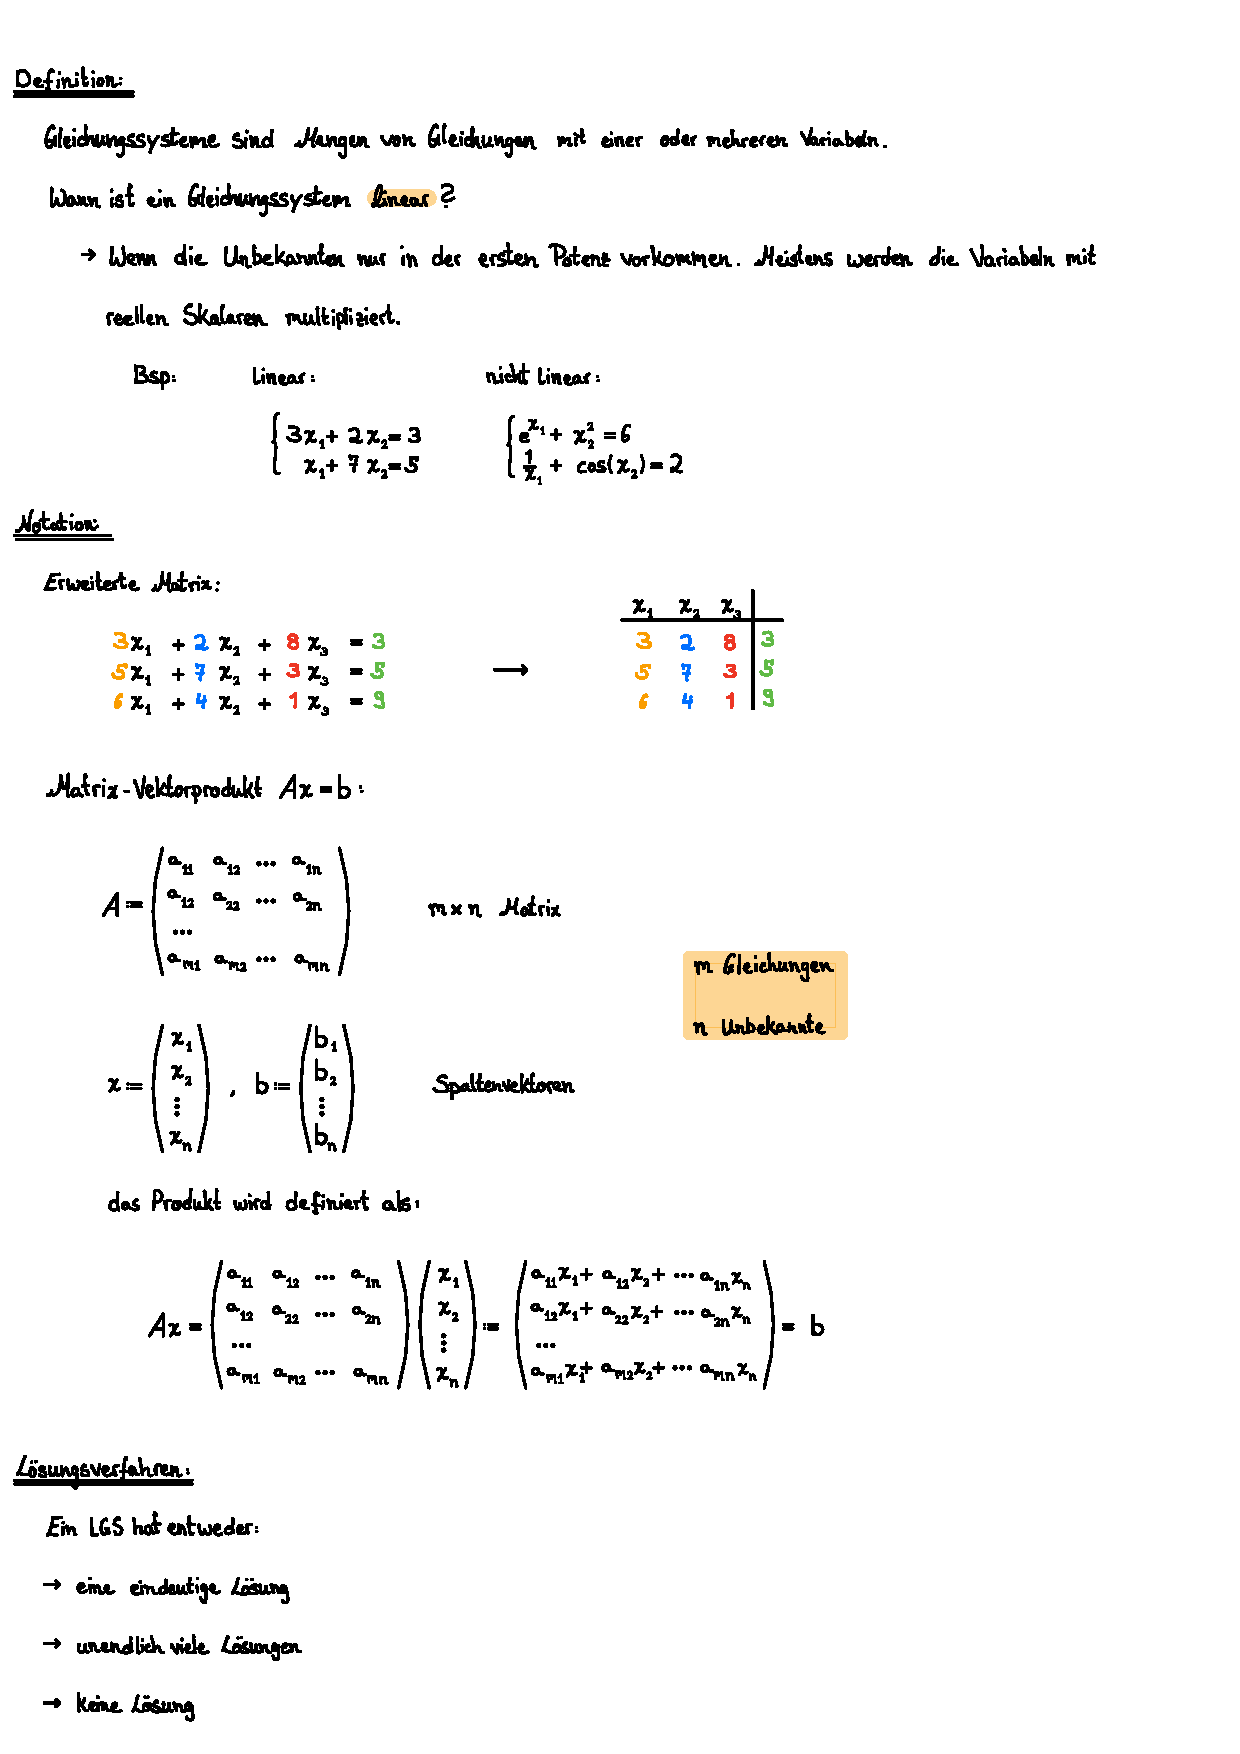
\includegraphics[page=1, scale=0.842]{pdf/01_Lineare_Gleichungssysteme.pdf}
\end{figure}
\newpage
\includepdf[pages={2-}, 
            pagecommand={\thispagestyle{plain}}, 
            scale=0.95]{pdf/01_Lineare_Gleichungssysteme.pdf}
            
\newgeometry{top=2.5cm, bottom=2cm}
\subsection{Beispielaufgaben}
\vspace{1cm}

\subsubsection{}  %Buch Seite 18 keine Lösungen
Für welche Werte des Parameters \( a \) hat das Gleichungssystem

\begin{equation*}
    \begin{aligned}
        a&x_1 +& 4&x_2 &+ 5x_3 &= a\\
        1&x_1 +& a&x_2 &- 2x_3 &= 1\\
        2&x_1 +& 2a&x_2 &- a^2x_3 &= a
    \end{aligned}   
\end{equation*}

keine, genau eine oder unendlich viele Lösungen? Bestimmen Sie jeweils auch die Lösungsmenge.

\vspace{1\baselineskip}

\begin{solution}

    \vspace{1\baselineskip}

    \leftskip=2em

    Gauss Verfahren anwenden:

    \begin{equation*}
        \begin{gmatrix}[L]
            a & 4 & 5 \\
            1 & a & -2 \\
            2 & 2a & -a^2
        \end{gmatrix} \hspace{-0.75em}
        \begin{gmatrix}[R]
            a \\ 1 \\ a
            \rowops
                \swap{0}{1}
        \end{gmatrix} \quad \rightarrow \quad
        \begin{gmatrix}[L]
            1 & a & -2 \\
            a & 4 & 5 \\
            2 & 2a & -a^2
        \end{gmatrix} \hspace{-0.75em}
        \begin{gmatrix}[R]
            1 \\ a \\ a
            \rowops
                \add[-a]{0}{1}
                \add[-2]{0}{2}
        \end{gmatrix} 
    \end{equation*}

    \vspace{1\baselineskip}

    \begin{equation*}
        \begin{gmatrix}[L]
            1 & a & -2 \\
            0 & -a^2 + 4 & 2a + 5 \\
            0 & 0 & 4 - a^2
        \end{gmatrix} \hspace{-0.75em}
        \begin{gmatrix}[R]
            1 \\ 0 \\ -2+a
        \end{gmatrix}
    \end{equation*}

    Nun können wir eine Fallunterscheidung machen:

    \vspace{1\baselineskip}

    \textbf{i}. keine Lösung: (Widerspruch in der letzten Zeile)
    \begin{equation*}
        \left.
        \begin{aligned}
            4 - a^2 &= 0 \; \Leftrightarrow \; a^2 = 4 \; \Leftrightarrow \; a = \pm 2\\
            -2 + a &\neq 0 \; \Leftrightarrow \; a \neq 2
        \end{aligned} \; \right\} \quad
        a = -2. 
    \end{equation*}

    \textbf{ii}. eindeutige Lösung: (keine Nullzeile, voller Rang)

    \begin{equation*}
        4-a^2 = -2+a \; \Leftrightarrow \; a^2+a-6 = 0 \; \Leftrightarrow \; (a-2)(a+3) = 0
    \end{equation*}

    Bei der Option \( a = 2 \) ist die letzte Zeile Null womit der Rang nicht voll ist. Es gilt also \( a = -3 \).

    \begin{equation*}
        \begin{gmatrix}[L]
            1 & -3 & -2 \\
            0 & -5 & -1 \\
            0 & 0 & -5
        \end{gmatrix} \hspace{-0.75em}
        \begin{gmatrix}[R]
            1 \\ 0 \\ -5
        \end{gmatrix} \quad \Rightarrow \quad
        \begin{aligned}
            x_3 &= 1 \\
            x_2 &= - \frac{x_3}{5} \; \Rightarrow \; x_2 = -\frac{1}{5} \\
            x_1 &= 1 + 3x_2 + 2x_3 \; \Rightarrow \; x_1 = \frac{12}{5}
        \end{aligned}
    \end{equation*}

    \textbf{iii}. unendlich viele Lösungen: (mindestens eine Nullzeile)
    
    \begin{equation*}
        \left.
        \begin{aligned}
            4 - a^2 &= 0 \; \Leftrightarrow \; a^2 = 4 \; \Leftrightarrow \; a = \pm 2\\
            -2 + a &= 0 \; \Leftrightarrow \; a = 2
        \end{aligned} \; \right\} \quad
        a = 2. 
    \end{equation*}

    \begin{equation*}
        \begin{gmatrix}[L]
            1 & 2 & -2 \\
            0 & 0 & 9 \\
            0 & 0 & 0
        \end{gmatrix} \hspace{-0.75em}
        \begin{gmatrix}[R]
            1 \\ 0 \\ 0
        \end{gmatrix} \quad \Rightarrow \quad
        \begin{aligned}
            x_3 &= 0 \\
            x_2 &= t, \; t \in \mathbb{R} \\
            x_1 &= 1 + 2x_3 - 2x_2 \; \Rightarrow \; x_1 = 1 - 2t
        \end{aligned}
    \end{equation*}

\end{solution}

\newpage

\subsubsection{} %Buch Seite 18 keine Lösungen

Geben Sie für \( a \) und \( b \) Bedingungen an, so dass das System

\begin{equation*}
    \begin{aligned}
        0 &x_1 &+ a &x_2 &+ 1 &x_3 &= -b\\
        a &x_1 &+ 0 &x_2 &+ b &x_3 &= -1\\
        a &x_1 &+ a &x_2 &+ 2 &x_3 &= -2
    \end{aligned}
\end{equation*}

\begin{enumerate}[label=\alph*)]
    \item eine Lösungsmenge mit \textit{zwei} freien Parametern besitzt.
    \item eine Lösungsmenge mit \textit{einem} freien Parameter besitzt.
    \item eindeutig lösbar ist.
    \item keine Lösung hat.
\end{enumerate}

Geben Sie sie für alle Fälle a), b), c) die Lösungsmenge an.

\vspace{1\baselineskip}

\begin{solution}    

    \vspace{1\baselineskip}

    \leftskip=2em

    Gauss Verfahren anwenden:

    \begin{equation*}
        \begin{gmatrix}[L]
            0 & a & 1 \\
            a & 0 & b \\
            a & a & 2
        \end{gmatrix} \hspace{-0.75em}
        \begin{gmatrix}[R]
            -b \\ -1 \\ -2
            \rowops
                \swap{0}{1}
        \end{gmatrix} \rightarrow \quad
        \begin{gmatrix}[L]
            a & 0 & b \\
            0 & a & 1 \\
            a & a & 2 
        \end{gmatrix} \hspace{-0.75em}
        \begin{gmatrix}[R]
            -1 \\ -b \\ -2
            \rowops
                \add[-1]{0}{2}
        \end{gmatrix} \rightarrow \quad
        \begin{gmatrix}[L]
            a & 0 & b \\
            0 & a & 1 \\
            0 & a & 2 - b
        \end{gmatrix} \hspace{-0.75em}
        \begin{gmatrix}[R]
            -1 \\ -b \\ -1
            \rowops
                \add[-1]{1}{2}
        \end{gmatrix}
    \end{equation*}

    \begin{equation*}
        \begin{gmatrix}[L]
            a & 0 & b \\
            0 & a & 1 \\
            0 & 0 & -b + 1
        \end{gmatrix} \hspace{-0.75em}
        \begin{gmatrix}[R]
            -1 \\ -b \\ b-1
        \end{gmatrix}
    \end{equation*}

    \vspace{1\baselineskip}

    \textbf{a)} Zwei freie Parameter: \( a = 0, \ b = 1\)

    \begin{equation*}
        \begin{gmatrix}[L]
            0 & 0 & 1 \\
            0 & 0 & 1 \\
            0 & 0 & 0
        \end{gmatrix} \hspace{-0.75em}
        \begin{gmatrix}[R]
            -1 \\ -1 \\ 0
        \end{gmatrix} \quad \Rightarrow \quad
        \begin{aligned}
            x_3 &= -1 \\
            x_2 &= t, \; t \in \mathbb{R} \\
            x_1 &= s, \; s \in \mathbb{R}    
        \end{aligned}
    \end{equation*}

    \textbf{b)} Ein freier Parameter: \( a \neq 0, \ b = 1\)

        \begin{equation*}
        \begin{gmatrix}[L]
            a & 0 & 1 \\
            0 & a & 1 \\
            0 & 0 & 0
        \end{gmatrix} \hspace{-0.75em}
        \begin{gmatrix}[R]
            -1 \\ -1 \\ 0
        \end{gmatrix} \quad \Rightarrow \quad
        \begin{aligned}
            x_3 &= t, \; t \in \mathbb{R} \\
            x_2 &= \frac{-1-t}{a} \\
            x_1 &= \frac{-1-t}{a}
        \end{aligned}
    \end{equation*}

    \textbf{c)} Eindeutig lösbar: \( a \neq 0, \ b \neq 1\)
    \begin{equation*}
        \begin{gmatrix}[L]
            a & 0 & b \\
            0 & a & 1 \\
            0 & 0 & -b + 1
        \end{gmatrix} \hspace{-0.75em}
        \begin{gmatrix}[R]
            -1 \\ -b \\ b-1
        \end{gmatrix} \quad \Rightarrow \quad
        \begin{aligned}
            x_3 &= -1\\
            x_2 &= \frac{b - 1}{a}\\
            x_1 &= \frac{b - 1}{a}
        \end{aligned}
    \end{equation*}

    \textbf{d)} Keine Lösung: \( a = 0, \ b \neq 1\)

\end{solution}